
\chapter{Priprema podataka} % Main chapter title

\label{Priprema_podataka} % For referencing 


\section{Objedinjavanje CAFA3 i novije Svis-Prot verzije}

Iz CAFA3 trening skupa izdvojeni su svi validni proteini ( dužine barem 9, i
azbukom od 20 standardnih aminokiselina). Ni u jednom trenutko ne izbacujemo
proteine kraće od 40 aminokiseline jer je to deo analize funkcije i nismo želeli
da ograničimo skup mogućih predikcija neuređenosti.

Informacije o Svis-Prot bazi dobijene su iz verzije 2017\_12, iz datoteke
\url{ftp://ftp.uniprot.org/pub/databases/uniprot/previous_releases/release-2017_12/knowledgebase/uniprot_sprot-only2017_12.tar.gz}.
Pomenuta verzija ima 556 196 proteina. 

Od 66 599 validnih CAFA3 proteina 66 530 ima nepromenjen \keyword{primarni
  identifikator} \en{accession number\footnote{Pod brojem se zapravo
  podrazumeva alfanumerička oznaka.}}.  69 novih unosa(slogova\footnote{ Slog
  \en{Record} u terminima baze podataka predstavlja zapis jednog elementa u
ovom slučaju reprezentacije proteina i njegovih karakteristika.  identifkovan
je primarnim identifikatorm.  }) u Svis-Prot bazu dobijena su revizijom CAFA3
proteina koji nam nedostaju.  Ovo je posledica dva moguća mehanizma:

\begin{enumerate}
  \item Unifikacija postojećih proteina u jedan novi slog. Rezultat ovog
    preslikavanja prikazan je na Slici \ref{fig:unifikacija_slogova}. Analizom
    ovih promena uspešno su rekonstruisana  svega 4 nova sloga. Kako je 4
    suviše mali broj zbog jednostavnosti zanemarili smo sve slogove dobijene
    unifikacijom.

  \begin{figure}[th]
  \centering
  
\includegraphics[scale=2]{plots/unifikacija_slogova2.eps}
  \decoRule
  \caption{Unifikacija starih(elipse) na nove slogove u Svis-Prot bazi}
  \label{fig:unifikacija_slogova}
  \end{figure}

  \item Specijalizacija jednog proteina u više različitih slogova.  Zbog moguće
    statističke redundantnosti ovi slogovi su zanemareni.
\end{enumerate}




Validini CAFA3 proteini anotirani su sa  5957 različitih GO termina Molekulske
Funkcije (MF) od kojih je 50 zamenjeno novijim terminom i izbačeno iz najnovije
\file{go.obo} datoteke. U Svis-Prot bazi nismo bili u mogućnosti da proverimo
za M,F ali ukupno je zamenjeno 319 GO termina.
CAFA3 sadrži 67 MF GO termina koji se ne javljaju u Swis-Prot anotacijama.
Swis-Prot sadrži 888 MF GO termina koji se ne javljaju u CAFA3 anotacijama.
Pošto Svis-Prot treba da sadrži svežije (tačnije) anotacije CAFA3 verzija
anotacija je zanemarena u koristi najnovijih Svis-Prot anotacija.

Pored anotacija Svis-Prot sadrži 194 proteina čija se sekvenca razlikuje u
odnosu na CAFA3 verziju proteina. Odlučeno je da ipak koristimo CAFA3 sekvence.

\section{Grupisanje proteina po GO terminima}

Anotacije ključnim rečima već podrazumevaju da će razmatranoj ključnoj reči
biti pridruženi i svi proteini specijalizovanijih ključnih reči. Kod GO
termina ovo nije slučaj. Ako termina A ''is\_a'' termin B onda i svi proteini
pridruženi A trebaju biti pridruženi terminu B. Tek nakon što je ovo grupisanje
odrađeno validno je odbaciti GO termine koji anotiraju manje od 20 proteina.
Za predloženo grupisanje korišćen je algoritam topološkog sortiranja.

\section{Ontologije gena i ključne reči}

U nastavku razmatramo samo ključne reči kategorije \keyword{molekulska
funkcija} i načine na koji ih možemo povezati na ekvivalentnim molekulskim
funkcijama GO termina.  Direktno mapiranje sa \keyword{ključnih reči} na GO
termine nije uvek moguće.  Neke ključne reči (Represor, Cyclin, Activator,
Superantigen, Tumorantigen ...) nemaju ''ekvivalentni'' GO termin. Od 226
ključnih reči svega 175 ima ''ekvivalentni'' GO termin. Od preostalih 175
postoji 105 mapiranja  na GO termin molekulske funkcije, 59 na biološke procese
i 11 na ćeliske komponente.  Dakle, za 70 ključnih reči kategorije molekulska
funkcija ne postoji direktno mapiranje na GO termin molekulske funkcije. Slika
\ref{fig:KWtop20dis} prikazuje sva moguća direktna mapiranja za 20 statistički
najznačajnijih neuređenih ključnih reči pronađenih u radu \parencite{Xie2007}.
U našoj verziji ključnih reči iz 2017 godine Antigen je izbačen i zamenjen
specijalizovanijom podelom. Tri ključne reči nemaju nikakvo mapiranje, dve se
mapiraju na ćeliske komponente, osam na biološke procese i svega šest na
molekulske funkcije.  Statistički značajne ključne reči su ljubičaste dok radi
kompletnosti navodimo neke njihove specijalizacije i generalizacije koje su
ofarbane sivo.

U nekim slučajevima GO biološkog procesa moguće je doći do molekulske funkcije
praćenjem veza ''je deo'' ili ''sadrži''. Međutim za 8 bioloških procesa ovo je moguće samo za Neuropeptid.
Dodatno ova metoda proizvodi diskutabilan rezultat. \keyword{Cypher} upitom:
\begin{verbatim}
MATCH p=(:Keyword {name:"Neuropeptide"})--(:GOTerm)<-[*0..]-(:GOTerm)<--(:Protein)
RETURN p
\end{verbatim}
pronađeno je mapiranje predstavljeno slikom \ref{fig:neuropeptide} na kojoj
se jasno vidi da se skupovi proteina anotirani molekulskom funkcijom
ne poklapaju sa skupom koje ključna reč Neuropeptid podrazumeva. Ovo je najverovatnije
posledica veze ''je deo'' koja ne podrazumeva kompoziciju (''sadrži'') već
samo agregaciju\footnote{ Relacija agregacije podrazumeva da molekulska
funkcija postoji nezavisno od biološkog procesa za razliku od relacije
kompozicije}. Kod ključnih reči od interesa veza ''sadrži'' ne postoji.

Dakle automatsko poređenje moguće je samo za šest od 20 originalnih neuređenih
ključnih reči. Za 20 uređenih ključnih reči postoji više mapiranja.  
Finalni metod koji smo koristili je poluautomatski. Od ključnih reči (od intersa)
ili njihovih delova napravljen je regularani izraz oblika:
\begin{verbatim}
  expresion = re.compile( f"({'|'.join(words)})[^ ,.)]*", re.I )
\end{verbatim}
Konstruisani regularan izraz iskorišćen je na sledeći način.  Prvo se pretražuje
da li se u imenu GO termina javlja zadata fraza.  Ako se ne javlja pretraga 
se proširuje na  sinonime GO termina. Ako ni tu nije pronađena pretraživanje se
proširuje na definiciju termina. Dobijene su tri vrste relacije opadajuće
pouzdanosti. Pažljivom ručnom analizom moguće je izvesti porđenje
rezultata. Ako su reči u frazi koju tražimo spojene sa povlakom ('-' karakterom)
onda to treba razdvojiti blanko karakterom jer GO termini gotovo nikad
ne sadrže povlaku osim možda u sinonimima. Najsigurnije je probati obe varijante.
Ovaj metod je uspešan zbog konzervativnosti fraza koje tražimo kao i informacije 
o sinonimima koje GO termini sadrže.






\begin{figure}[th]
\hspace*{-2.2cm} 
\includegraphics[scale=1]{Figures/plots/kw_dis2go.pdf}
\decoRule
\caption {
  Mapiranje 20 statistički najznačajnijih neuređenih molekulskih funkcija \parencite{Xie2007} 
  na GO termine.
}
\label{fig:KWtop20dis}
\end{figure}


\begin{figure}[th]
\centering
\hspace*{-2.2cm} 
\includegraphics[scale=0.9]{Figures/plots/Neuropeptide2go.pdf}
\decoRule
\caption {
  Slika prikazuje da direktno mapiranje sa ključne reči na GO istog imenskog prostora (kategorije) nije uvek direktno.
  Takođe ovako postignuta mapiranja dele mali broj zajedničkih proteina.
}
\label{fig:neuropeptide}
\end{figure}
